\chapter{Fatiando a Terra}

\section{Resumen}


\section{Introducción}

% Necesidad de software open-source en geofísica.

Desde su invención, las computadoras han sido puestas a disposición de la
comunidad científica con el objetivo de resolver problemas que resultaban
inalcanzables.
Esta interacción entre una tecnología de vanguardia y el ambiente científico
generaba no solo beneficios para esta última parte, sino también una gran
retroalimentación.
Se desarrollaron lenguajes de programación especialmente diseñados para
resolver problemas numéricos junto con interfaces que facilitaran la
visualización y manipulación de datos científicos.
La relación entre ciencia y las herramientas computacionales se desarrolló tan
rápido que fue necesario crear el término \emph{computación científica} para
diferenciarla de los otros usos que se estaban gestando para las computadoras
(telecomunicaciones, fines comerciales, sistemas estatales de datos, etc.).
Hoy en día es imposible imaginar una ciencia que no necesite de las
herramientas computacionales para su avance y la resolución de los problemas
actuales que enfrenta.

A medida que los problemas científicos se vuelven cada vez más complejos de
resolver, las tareas científicas de aprender los últimos conocimientos en la
materia, adquirir nuevos datos, desarrollar el software necesario para
procesarlos y finalmente generar un nuevo conocimiento, se presenta como un
desafío titánico para ser desempeñado por una persona o por apenas un puñado de
investigadores.
La complejidad actual de la ciencia requiere que el clásico flujo de trabajo
científico se distribuya a lo ancho de la comunidad, ofreciendo productos
o soluciones para cada una de sus etapas, que puedan ser utilizados libremente
por otros investigadores y otras investigadoras, que a su vez puedan
modificarlos y volver a distribuirlos en caso de desearlo.
En resumen, los problemas científicos actuales requieren soluciones
comunitarias, tanto para dar respuestas a las preguntas fundamentales, así como
para desarrollar herramientas que faciliten la resolución de estos problemas.

Por fuera de la comunidad científica (aunque con algunas intersecciones) se
comenzó a gestar en la década del 80 un movimiento que trabajaba en la creación
de herramientas computaciones con características similares.

Movimiento open-source en ciencia (iPython, Jupyter, Numpy, Matplotlib,
Astropy, etc), estado actual.


\section{Historia}

Los orígenes del proyecto se remonta a finales de la década del 2000, cuando
Leonardo Uieda, Vanderlei Oliveira Jr. junto a otros estudiantes se encontraban
cursando los últimos años del Bachillerato en Geofísica (\emph{Bacharelado em
Geofísica}) en la Universidade de São Paulo.
En este contexto surge la idea de implementar una alternativa propia a los
software de modelado gravimétrico 2D comerciales.
Tras asistir a cursos dictados por
Software Carpentry\footnote{%
    \url{https://software-carpentry.org}
}
en Canadá, Leonardo Uieda adquiere mayores conocimientos en el uso de sistema
de control de versiones junto a otras mejores prácticas para el desarrollo de
Software, regresa con nuevas ideas para el proyecto y un diagrama de un posible
diseño para este proyecto (fig.~\ref{fig:talwani-idea}).
La idea finalmente se desarrolla mediante
una implementación del método de \citet{talwani1959} para
modelado directo de polígonos 2D, y la posterior construcción de una interfaz
gráfica escrita en C que más tarde se reimplementaría en Python.

\begin{figure}
    \centering
    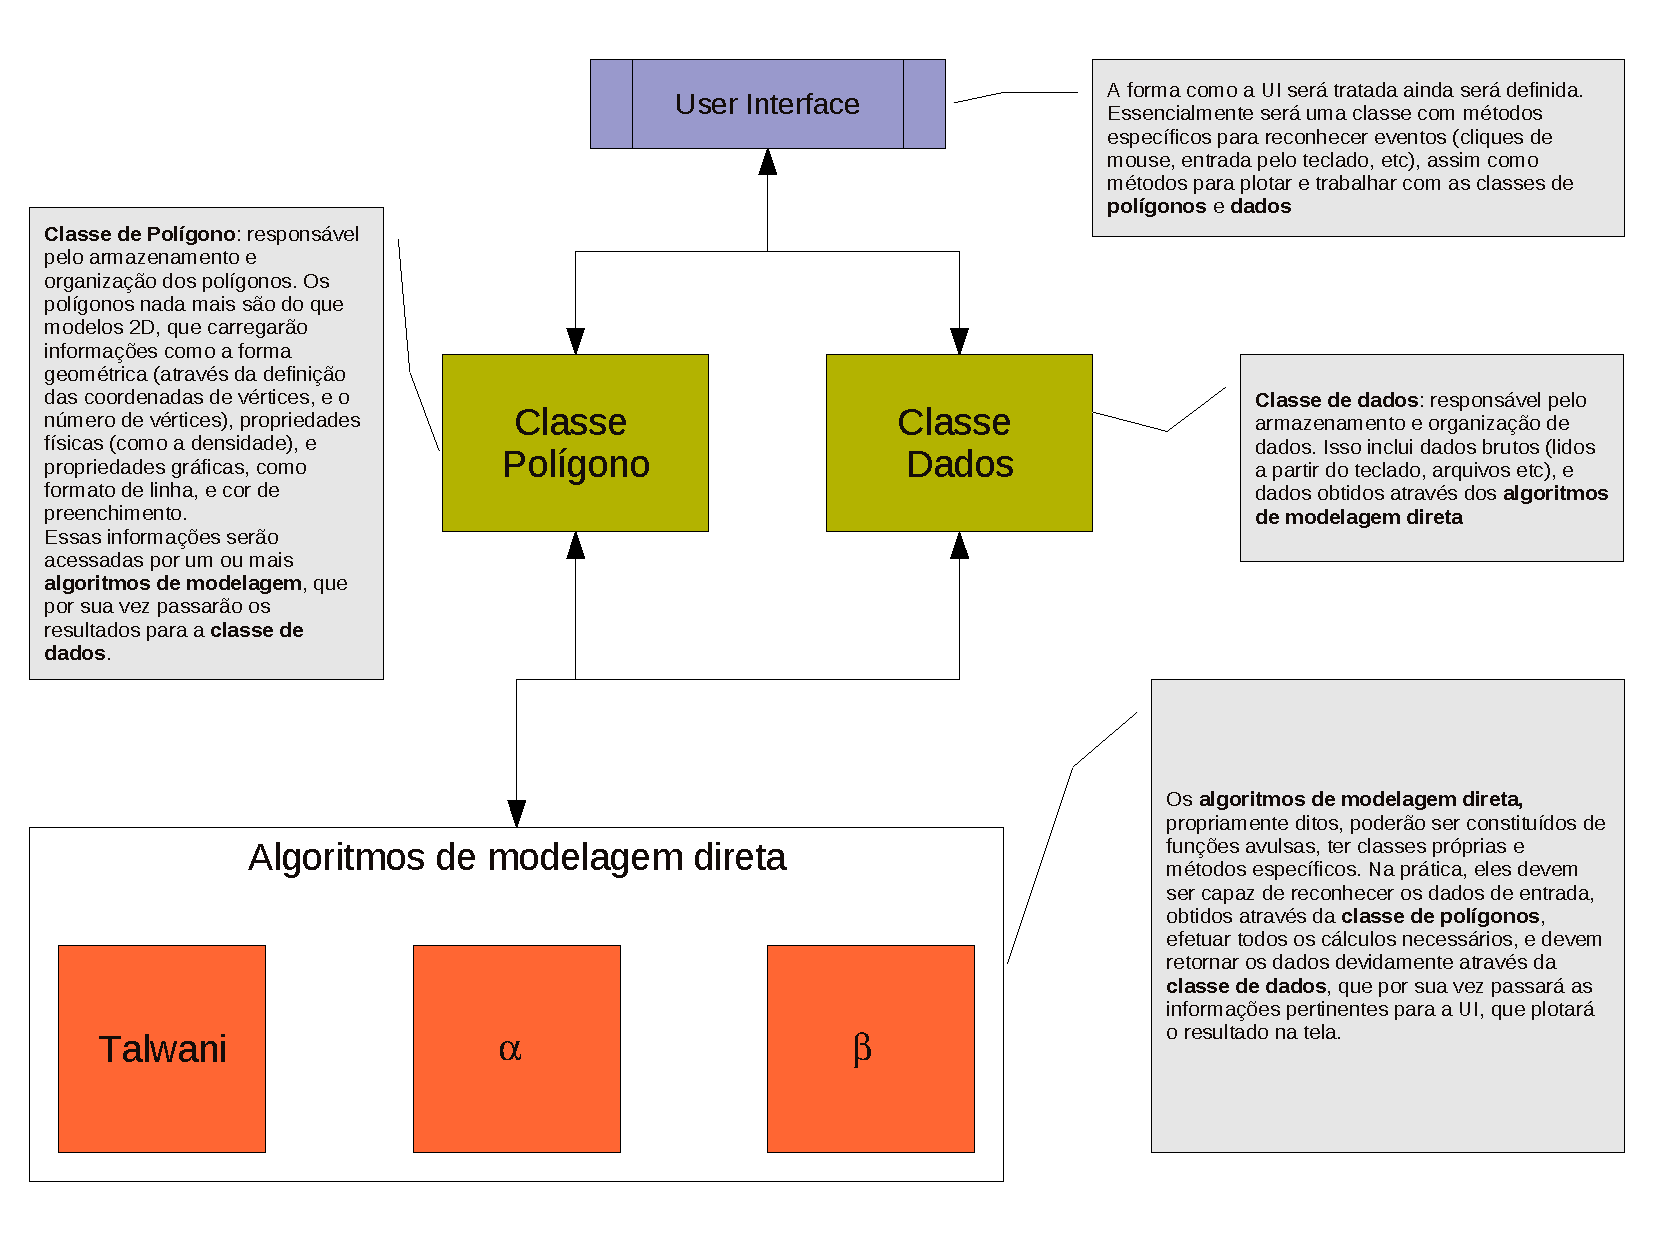
\includegraphics[width=\linewidth]{figs/fluxo-simples.pdf}
    \caption{
        Diagrama de flujo para la primera implementación de un software para el
        modelado gravimétrico de polígonos 2D. Realizado por Leonardo Uieda
        (circa 2009).
    }
    \label{fig:talwani-idea}
\end{figure}

En paralelo, y como proyecto final de su Bachillerato, Leonardo Uieda realiza
una implementación en Python del algoritmo para el cálculo de campos
gravitacionales de tesseroides mediante la \ac{GLQ}.
Luego de reescribirlo en C, este proyecto deriva en el lanzamiento del software
Tesseroids \citep{uieda2016} que ha sido ampliamente utilizado por la comunidad
geocientista.

El éxito de estos proyectos los llevó a aspirar a una idea mucho más
ambiciosa: desarrollar un software de código abierto para modelar el planeta
Tierra de
forma completa.
En ese entonces surge un nombre para el proyecto: \emph{Fatiando a Terra}, que
puede traducirse como \emph{rebanando la Tierra}.

Durante su Master en Geofisica en el Observatório Nacional, Rio de Janeiro,
Leonardo comienza el desarrollo de Fatiando a Terra, transformándolo en el hogar
de las implementaciones que realiza a lo largo de sus investigaciones, todas
mediante el lenguaje Python.
Entre ellas podemos encontrar: modelados directos con diferentes geometrías,
continuación ascendente, deconvolución de Euler, fuentes equivalentes, hasta un
incipiente \emph{framework} de inversión y algunas implementaciones de
tomografías sísmicas simples.

En los años posteriores, cuando la mayoría de los gestores del proyecto se
encontraban cursando sus Doctorados, Fatiando a Terra comienza a cobrar mayor
forma.
Leonardo y Vanderei deciden utilizar el \emph{framework} de inversión para dar
un curso sobre inversiones geofísicas en la Universidade de São Paulo.
Fatiando adquiere su propio dominio
(\href{https://www.fatiando.org}{fatiando.org}) y su primera página web,
alojada en un servidor casero por José Caparica Jr\footnote{%
    Más adelante se utilizarán los servicios de
    \href{https://readthedocs.org/}{Read The Docs} para alojar el sitio web,
    que más tarde se reemplazarían por GitHub Pages.
}.
Además se elige distribuirlo bajo la licencia
\href{https://opensource.org/licenses/BSD-3-Clause}{BSD 3-clause}.
En 2013, el proyecto es presentado en una charla en SciPy 2013
\citep{uieda2013}.

En los años posteriores el proyecto comienza a cobrar mayor reconocimiento.
Empieza a ser utilizado en publicaciones científicas
\citep[][entre otros]{%
    uieda2012,
    carlos2014,
    oliveira2015,
    hidalgogato2015,
    carlos2016,
    reis2016,
    uieda2017,
    hidalgogato2017,
    siqueira2017%
},
% fill in more papers if you know about some others
dictado de clases
(Tópicos de inversão em
geofísica\footnote{%
    \url{https://www.leouieda.com/teaching/inversao-iag-2012.html}
    y \url{https://www.leouieda.com/teaching/inversao-unb-2014.html}
},
\citet{uieda2014},
Geofísica 1: Gravimetria e magnetometria\footnote{%
    \url{https://www.leouieda.com/teaching/geofisica1.html}
},
Geofísica 2: Sismologia e sísmica\footnote{%
    \url{https://www.leouieda.com/teaching/geofisica2.html}
})
y en trabajos finales de grado y posgrado
\citep{carlos2013, sales2014, soler2015, uieda2016b, melo2020}.
Además comienza a atraer la atención de la comunidad internacional, recibiendo
colaboraciones de investigadores y desarrolladores de diferentes partes del
mundo.
La utilización de fatiando por otros investigadores e investigadoras deriva
a su vez en un ciclo de retroalimentación: quienes comienzan siendo usuarios
realizan colaboraciones.
De esta forma fatiando comienza a alojar implementaciones de métodos
novedosos recientemente publicados \citep{uieda2012b, oliveira2013}.

Mi primea contribución al proyecto consistió en una implementación del promedio
radial del espectro de frecuencias de grillas de gravedad
o magnetismo\footnote{%
    \url{https://github.com/fatiando/fatiando/pull/303}
}.
Desde entonces comencé a involucrarme cada vez más en el proyecto, lo que me
permitió adquirir mayores conocimientos en el uso de controladores de
versiones, flujos de trabajo para el desarrollo colaborativo, creación de
funciones de \emph{testing}, buenas prácticas para el diseño de algoritmos y la
importancia de mantener la documentación actualizada.

La última versión del paquete fatiando es la v0.5, lanzada en Noviembre de
2016.
Si bien ese paquete en particular se encuentra obsoleto y no recibe mayor
mantenimiento, esto no significa que la vida de el proyecto haya finalizado en
ese entonces.

A partir de 2018 el proyecto tomó una nueva dirección.
El panorama de software de código abierto para Geofísica había cambiado mucho
desde los inicios de Fatiando a Terra: la cantidad de nuevos paquetes diseñados
para atacar diversos problemas de las geociencias había aumentado
considerablemente
\citep{cockett2015, ruecker2017, varga2019, obspy2019}.
Dentro de este nuevo ecosistema, fatiando no poseía un objetivo claro.
Esto no solo hacía difícil que potenciales usuarios y usuarias identifiquen el
propósito del proyecto, sino que también constituía una base de código difícil
de mantener.
Por otro lado, para ese entonces fatiando había sido el hogar de
implementaciones de métodos clásicos de la geofísica, métodos muy novedosos
(orientados principalmente a la investigación científica), así como de código
\emph{juguete} diseñado para ser utilizado en clases para fines didácticos
pero sin las capacidades para atacar problemas reales.
Sumado a esto, la versión de Python 2.7 llegaba pronto a su final de vida, lo
que hacía necesario adaptar fatiando al nuevo Python 3.

Estas razones ponían en evidencia la necesidad de establecer objetivos claros
para el proyecto, así como también repensar su diseño y sustentabilidad
a futuro.
Por esto se tomó la decisión de dividir el proyecto en varios paquetes que
posean objetivos claros y concisos.
Esto permitiría no sólo una fácil adopción por parte de usuarios y usuarias,
sino también que otros proyectos los utilicen como dependencias en caso de
desearlo.
Además, manteniendo los campos de acción de cada paquete aislados del resto,
se facilitaría el desarrollo a futuro: los colaboradores no necesitan
familiarizarse con el proyecto completo, sino solo con algunas de sus partes.
Por otro lado, la decisión de reescribir gran parte del código se presentó como
una oportunidad para pensar mejores diseños del software ya existente y de
implementar mejores
prácticas para el desarrollo de software, estableciendo estándares de calidad
más altos.


\section{Paquetes de software}

Actualmente Fatiando a Terra está compuesto por cuatro paquetes de software
destinados a ofrecer soluciones a diversas problemáticas en geociencias, así
como también a otras áreas de la ciencia:

\begin{description}
    \item[\emph{Verde}]{%
        Procesado y grillado de datos espaciales
    }
    \item[\emph{Boule}]{%
        Elipsoides de referencia para aplicaciones geodésicas y geofísicas
    }
    \item[\emph{Harmonica}]{%
        Procesado, modelado directo e inverso de datos gravimétricos
        y magnéticos
    }
    \item[\emph{Pooch}]{%
        Descargar y almacenar datos científicos de la web de forma sencilla
    }
\end{description}

\subsection{Verde}

\emph{Verde} ofrece herramientas para procesar datos espaciales (tales como
muestras geofísicas obtenidas en el campo, mediciones de batimetría, etc)
e interpolarlos sobre grillas regulares.

La mayoría de los muestreos de datos espaciales se componen por datos
irregularmente distribuidos sobre la zona de estudio:
puntos dispersos, trayectos irregulares o líneas casi rectas.
Sin embargo, muchas metodologías de procesado e interpretación requieren que
los datos se sitúen sobre puntos pertenecientes a una grilla regular.
Este problema suele resolverse mediante la interpolación de los datos
originales sobre una grilla regular, proceso que se conoce como
\emph{grillado}.

Dentro de los algoritmos de grillado existe una categoría que se conoce como
\emph{interpolaciones con funciones de base radial} (\emph{radial basis
function interpolation} en inglés). Un ejemplo de un algoritmo que entra en
esta categoría son las \emph{splines} biharmónicas.
Estos métodos asumen que podemos representar los datos observados por una
combinación lineal de funciones de Green, es decir:

\begin{equation}
    d_i = \sum_{j=1}^M c_j G(\mathbf{p}_i, \mathbf{q}_j),
\end{equation}

\noindent donde $d_i$ y es el dato $i$-ésimo, $\mathbf{p}_i$ es la ubicación de
ese mismo punto, $c_j$ es un coeficiente escalar, $G$ es una función de Green y
$\mathbf{q}_j$ es la ubicación del punto que define la función de Green en el
término $j$-ésimo.
El proceso de interpolación consiste en ajustar los valores de los
coeficientes $c_j$ mediante mínimos cuadrados de forma tal que se recuperen los
datos observados, y luego utilizarlos para predecir valores sobre los puntos de
la grilla:

\begin{equation}
    d(\mathbf{p}) = \sum_{j=1}^M c_j G(\mathbf{p}, \mathbf{q}_j),
\end{equation}

\noindent donde $\mathbf{p}$ es la ubicación de cualquier punto de la grilla.

Dentro de \emph{Verde} hallamos implementaciones de algoritmos de interpolación
de este tipo siguiendo un diseño similar
a los modelos de aprendizaje automático de \emph{scikit-learn}
\citep{sklearn2011}. Esto permite que quienes estén familiarizados con la
aplicación de métodos de aprendizaje automático en Python puedan fácilmente
entender cómo utilizar la \ac{API} de \emph{Verde}.
Entre los algoritmos de interpolación que se encuentran implementados están las
\emph{splines} biharmónicas, así como métodos más complejos como la
interpolación de vectores 2D con funciones de Green \citep{sandwell2016}.

Como hemos mencionado anteriormente, los interpoladores presentes en
\emph{Verde} han sido implementados mediante clases que reproducen un
comportamiento similar a las clases de \emph{scikit-learn}.
Los interpoladores en verde poseen un método \texttt{fit()} que se usa para
ajustar los parámetros $c_j$ mediante mínimos cuadrados partiendo de un
conjunto de datos y sus ubicaciones. Luego podemos hacer uso del método
\texttt{predict()} para predecir valores en cualquier conjunto de puntos,
o bien usando el método \texttt{grid()} podemos predecir sobre una grilla
regular de puntos.

Además, \emph{Verde} cuenta con utilidades para realizar reducciones por
bloque, una clases para determinación de tendencias polinomiales, funciones
para el manejo de coordenadas, y herramientas para realizar validaciones
cruzadas y selección de modelos.

El diseño de \emph{Verde} permite su extensibilidad: todos los interpoladores
heredan su estructura a partir de una clase base denominada
\texttt{verde.BaseClass}, lo cual permite construir nuevos tipos de
interpoladores de manera sencilla, restando que definir únicamente el tipo de
función de Green a utilizar.
Además, debido a la compatibilidad con las librerías científicas de Python, es
posible integrarlo a flujos de trabajos establecidos con gran facilidad.

La versión v1.0.0 de \emph{Verde} ha sido publicada en el Journal of Open
Source Software luego de un proceso abierto de revisión por pares
\citep{verde2018}.
Podemos acceder a la documentación correspondiente a la última versión estable
de la librería en \href{https://www.fatiando.org/verde}{fatiando.org/verde}.


\subsection{Boule}

\emph{Boule} es una librería que nos permite representar elipsoides de
referencia mediante objetos. Además nos ofrece herramientas para calcular los
campos gravitatorios que estos elipsoides generan y para realizar conversiones
de coordenadas.

Como hemos visto en la sección~\ref{sec:gravedad-terrestre}, un elipsoide de
referencia puede definirse mediante los semiejes mayor $a$ y menor $b$, su masa
total $M$ y su velocidad angular $\omega$.
De forma alternativa pero equivalente, es posible definirlo mediante los
siguientes parámetros:

\begin{itemize}
    \item el semieje mayor $a$,
    \item el achatamiento $f = (a - b) / a$,
    \item la constante gravitacional geocéntrica $GM$ (donde $M$ es la masa
        del elipsoide y $G$ la constante de gravitación universal),
    \item y la velocidad angular $\omega$.
\end{itemize}

Las funcionalidades principales de \emph{Boule} vienen dadas dentro de la clase
\texttt{Ellipsoids}, la cual nos permite definir cualquier elipsoide de
referencia a partir de los parámetros mencionados.
A modo de ejemplo, uno podría definir el elipsoide WGS84 como se muestra en le
Código~\ref{lst:boule-wgs84}.
Sin embargo, \emph{Boule} ya ofrece algunos de los elipsoides de referencia más
ampliamente usados en geodesia y geofísica, tales como el WGS84
(\texttt{boule.WGS84}), el GRS80: Geodetic Reference System
(\texttt{boule.GRS80}) e incluso un elipsoide de referencia para el planeta
Marte definido según los parámetros disponibles en \citet{ardalan2009}
(\texttt{boule.MARS}).

\lstinputlisting[
    float,
    language=Python,
    caption={Ejemplo de definición de elipsoide de referencia con \emph{Boule}},
    label=lst:boule-wgs84
]{chapters/fatiando-examples/boule-wgs84.py}

A su vez, la clase \texttt{Ellipsoids} posee una serie de propiedades que se
calculan a partir de los parámetros que definen cada elipsoide, entre ellos: el
semieje menor $b$, la primera y segunda excentricidad, la excentricidad lineal,
el radio medio del elipsoide (medido desde un sistema geocéntrico), el módulo
del vector aceleración de la gravedad sobre cualquier punto en el ecuador o en
sus polos.
Además, la misma clase ofrece un conjunto de métodos útiles para realizar
cálculos acerca de los campos gravitatorios que genera el elipsoide
y conversión de unidades.
El método \texttt{geocentric\_radius()} nos permite calcular la distancia entre
el centro del elipsoide y cualquier punto de su superficie a partir de su
latitud geodésica o geocéntrica.
Los métodos \texttt{geodetic\_to\_spherical()}
y \texttt{spherical\_to\_geodetic()} nos permiten convertir coordenadas
geodésicas en esféricas geocéntricas o viceversa siguiendo las ecuaciones de
\citet{vermeille2002}.
El método \texttt{normal\_gravity()} implementa la \emph{fórmula cerrada} de
\citet{li2001a} para calcular el módulo de la aceleración de la gravedad
generada por el elipsoide en cualquier punto dado por sus coordenadas
geodésicas.

Si bien \emph{Boule} es una librería que se encuentra en un estado funcional
y puede ser utilizada en investigaciones científicas al día de la fecha, aún no
ha alcanzado su primera versión estable.
Es posible que aún sea necesario realizar modificaciones sobre su diseño en los
planes de incorporar otros tipos de elipsoides, como las esferas o elipsoides
triaxiales.
A pesar de ello, podemos acceder a la documentación correspondiente a la última
versión lanzada en \href{https://www.fatiando.org/verde}{fatiando.org/boule}.


\subsection{Harmonica}

\subsection{Pooch}

\emph{Pooch} nos ofrece herramientas para descargar datos científicos alojados
en Internet, almacenarlos localmente y comprobar sus sumas de verificación,
entre otras características.

Muchas de las librerías de software científico hacen uso de datos de muestra
para ejemplificar su funcionamiento en las secciones de la documentación que se
conocen como \emph{Galería de ejemplos}.
Usualmente estos datos de muestra se incluyen dentro de los repositorios donde
se aloja el mismo código fuente de la librería, sin embargo estos archivos de
datos no son empaquetados para su distribución con el objetivo de reducir el
tamaño de las futuras instalaciones.
En cambio, los datos de muestra suelen ser descargados al ser necesarios
mediante código implementado dentro de cada una de estas librerías, haciendo
uso de paquetes de Python para descargar archivos mediante protocolo HTTP por
ejemplo.
\emph{Pooch} surge como una solución a este problema transversal a muchas
librerías del ecosistema científico de Python.

\lstinputlisting[
    float,
    language=Python,
    caption={%
        Ejemplo de descarga de archivos con \emph{Pooch} mediante la
        clase \texttt{pooch.Pooch}. Este código es a modo de ejemplificación
        y no está escrito para ser ejecutado.
    },
    label=lst:pooch-registry
]{chapters/fatiando-examples/pooch-registry.py}


\emph{Pooch} permite gestionar un \emph{registro} en el cual podemos listar las
direcciones de cada uno de los archivos que queremos ofrecer para su descarga,
junto con el \emph{hash} de una suma de verificación. Al solicitar alguno
o algunos de estos archivos, \emph{Pooch} se encarga de descargarlos de su
correspondiente localización, almacenarlos en un \emph{caché} local y realizar
una suma de verificación con el objetivo de certificar la integridad de los
mismos.
La descarga de los archivos se lleva a cabo únicamente si no existe tal archivo
en el \emph{caché} local.
En el Código~\ref{lst:pooch-registry} podemos visualizar cómo es posible
utilizar la función \texttt{pooch.create()} para inicializar una instancia de
la clase \texttt{pooch.Pooch} especificando el directorio donde se descargarán
los archivos, la dirección base donde se encuentran alojados los archivos de
interés, y el \emph{registro} donde especificamos el nombre de los archivos
y sus \emph{hashes} de las sumas de verificación.
Luego podemos solicitar la descarga de uno de los archivos mediante el método
\texttt{fetch()}, el cual devuelve la ruta al archivo descargado y almacenado
localmente.

\emph{Pooch} no sólo nos permite descargar archivos desde el protocolo HTTPS,
sino también desde FTP y SFTP con autenticación.
Incluso es posible descargar archivos almacenados en repositorios de acceso
abierto como Zenodo\footnote{\url{https://zenodo.org/}}
o figshare\footnote{\url{https://figshare.com}} únicamente mediante el
\ac{DOI}.
A su vez, también soporta diferentes tipos de suma de verificación, como
SHA256, MD5, XXH128, entre otras.
Además ofrece la posibilidad de realizar post-procesados luego de la descarga
de los archivos, como por ejemplo descomprimir archivos \texttt{.zip},
\texttt{.tar}, \texttt{.gzip}, \texttt{.xz}, etc.

El paquete presenta ciertas cualidades que lo hacen un excelente candidato para
ser utilizados por librerías de terceros.
En primer lugar, es posible configurarlo para que se adapte a diferentes
necesidades en pocas líneas con una sintaxis sencilla.
En segundo lugar, es un paquete puramente escrito en Python con dependencias
mínimas.
Y por último, presenta un alto grado de extensibilidad: es posible definir
funciones propias para otro tipos de descargas (desde otros protocolos, por
ejemplo) o bien para realizar post-procesados. Estas funciones personalizadas
puede acoplarse fácilmente al \emph{framework} de \emph{Pooch}, permitiendo
utilizar su misma sintaxis y sus capacidades de descarga, almacenamiento
y comprobación de sumas de verificación, incluso en aplicaciones particulares.

La versión v0.7.1 de \emph{Pooch} fue publicada en el Journal of Open Source
Software luego de una revisión abierta por pares \citep{pooch2020}.

\lstinputlisting[
    float,
    language=Python,
    caption={%
        Ejemplo de descarga de archivos con \emph{Pooch} mediante la
        función \texttt{pooch.retrieve()}.
    },
    label=lst:pooch-retrieve
]{chapters/fatiando-examples/pooch-retrieve.py}

Hasta entonces la principal audiencia de \emph{Pooch} eran otros
desarrolladores de software que deseaban una forma sencilla de distribuir datos
de muestra a sus usuarios.
Sin embargo, en los meses subsiguientes se presentó la oportunidad de incluir
otro tipo de audiencia al paquete: usuarios finales que deseaban descargar
pocos archivos por única vez.
Esto se materializó con la creación de la función \texttt{pooch.retrieve()} que
permite acceder a las mismas funcionalidades de \emph{Pooch}, pero sin la
necesidad de predefinir una instancia de \texttt{pooch.Pooch} y con una
interfaz más sencilla.
El Código~\ref{lst:pooch-retrieve} ejemplifica cómo podemos utilizar la función
\texttt{pooch.retrieve()} para descargar un archivo, almacenarlo localmente
y comprobar su suma de verificación en una única ejecución.
La función devuelve la ruta al archivo descargado y almacenado localmente.

% quien usa pooch hoy en dia
% xarray
% scikit-image

\section{Desarrollo y mejores prácticas}
\label{sec:best-practices}

Flujo de trabajo en Github.

Code review.

Documentación.

Testeo.

CI.

Ejemplos.

Filosofía UNIX?

Releases y backward compatibility?

Pypi y conda-forge?


\section{Comunidad}

Codigo de conducta

Instructivos para contribuir

Reuniones periodicas

Discusiones abiertas en issues/PRs

Interacción con otros proyectos?


\section{Adopción en la comunidad científica}

Publicaciones científicas relacionadas.

Tutoriales en Transform2020 y Transform 21 charla para la GSH

Visitas a la página web


\section{Planes a futuro}

Stable release of every package

Mayor interoperabilidad con el resto de paquetes geofísicos (SimPEG, pyGIMLi, etc)

Implementar esféras en boule (luna, mercurio).
Implementar elipsoides traixiales en boule.
Unificar las clases de elipsoides para todo tipo.
